\upaper{173}{Monday in Jerusalem}
\uminitoc{Cleansing the Temple}
\uminitoc{Challenging the Master’s Authority}
\uminitoc{Parable of the Two Sons}
\uminitoc{Parable of the Absent Landlord}
\uminitoc{Parable of the Marriage Feast}
\author{Midwayer Commission}
\vs p173 0:1 Early on this Monday morning, by prearrangement, Jesus and the apostles assembled at the home of Simon in Bethany, and after a brief conference they set out for Jerusalem. The twelve were strangely silent as they journeyed on toward the temple; they had not recovered from the experience of the preceding day. They were expectant, fearful, and profoundly affected by a certain feeling of detachment growing out of the Master’s sudden change of tactics, coupled with his instruction that they were to engage in no public teaching throughout this Passover week.
\vs p173 0:2 As this group journeyed down Mount Olivet, Jesus led the way, the apostles following closely behind in meditative silence. There was just one thought uppermost in the minds of all save Judas Iscariot, and that was: What will the Master do today? The one absorbing thought of Judas was: What shall I do? Shall I go on with Jesus and my associates, or shall I withdraw? And if I am going to quit, how shall I break off?
\vs p173 0:3 It was about 9:00 on this beautiful morning when these men arrived at the temple. They went at once to the large court where Jesus so often taught, and after greeting the believers who were awaiting him, Jesus mounted one of the teaching platforms and began to address the gathering crowd. The apostles withdrew for a short distance and awaited developments.
\usection{Cleansing the Temple}
\vs p173 1:1 A huge commercial traffic had grown up in association with the services and ceremonies of the temple worship. There was the business of providing suitable animals for the various sacrifices. Though it was permissible for a worshipper to provide his own sacrifice, the fact remained that this animal must be free from all “blemish” in the meaning of the Levitical law and as interpreted by official inspectors of the temple. Many a worshipper had experienced the humiliation of having his supposedly perfect animal rejected by the temple examiners. It therefore became the more general practice to purchase sacrificial animals at the temple, and although there were several stations on near\hyp{}by Olivet where they could be bought, it had become the vogue to buy these animals directly from the temple pens. Gradually there had grown up this custom of selling all kinds of sacrificial animals in the temple courts. An extensive business, in which enormous profits were made, had thus been brought into existence. Part of these gains was reserved for the temple treasury, but the larger part went indirectly into the hands of the ruling high\hyp{}priestly families.
\vs p173 1:2 This sale of animals in the temple prospered because, when the worshipper purchased such an animal, although the price might be somewhat high, no more fees had to be paid, and he could be sure the intended sacrifice would not be rejected on the ground of possessing real or technical blemishes. At one time or another systems of exorbitant overcharge were practised upon the common people, especially during the great national feasts. At one time the greedy priests went so far as to demand the equivalent of the value of a week’s labour for a pair of doves which should have been sold to the poor for a few pennies. The “sons of Annas” had already begun to establish their bazaars in the temple precincts, those very merchandise marts which persisted to the time of their final overthrow by a mob three years before the destruction of the temple itself.
\vs p173 1:3 \pc But traffic in sacrificial animals and sundry merchandise was not the only way in which the courts of the temple were profaned. At this time there was fostered an extensive system of banking and commercial exchange which was carried on right within the temple precincts. And this all came about in the following manner: During the Asmonean dynasty the Jews coined their own silver money\fnst{\textbf{Jews coined their own silver money}, The ``Jewish money'' proper, coined during the years of Hasmonean dynasty (164\,--\,35\,B.C.) should not be confused with the Tyrian type half-shekels required for the Temple tax and other offerings (cf.~Mishna Bek.8.7) and probably minted in Jerusalem after the mint in Tyre was closed down by Rome in 19\,B.C. The Hasmonean money (so far only bronze coins have been found) never contained images of gods or people or animals, like the Tyrian silver shekels and half-shekels (see the picture).}, and it had become the practice to require the temple dues of ½ shekel and all other temple fees to be paid with this Jewish coin. This regulation necessitated that money\hyp{}changers be licensed to exchange the many sorts of currency in circulation throughout Palestine and other provinces of the Roman Empire for this orthodox shekel of Jewish coining. The temple head tax, payable by all except women, slaves, and minors, was ½ shekel, a coin about the size of a 10¢ piece but twice as thick. By the times of Jesus the priests had also been exempted from the payment of temple dues. Accordingly, from the 15\ts{th} to the 25\ts{th} of the month preceding the Passover, accredited money\hyp{}changers erected their booths in the principal cities of Palestine for the purpose of providing the Jewish people with proper money to meet the temple dues after they had reached Jerusalem. After this 10\hyp{}day period these money\hyp{}changers moved on to Jerusalem and proceeded to set up their exchange tables in the courts of the temple. They were permitted to charge the equivalent of from 3¢ to 4¢ commission for the exchange of a coin valued at about 10¢, and in case a coin of larger value was offered for exchange, they were allowed to collect double. Likewise did these temple bankers profit from the exchange of all money intended for the purchase of sacrificial animals and for the payment of vows and the making of offerings.\tunemarkup{pictures}{\begin{figure}[H]\centering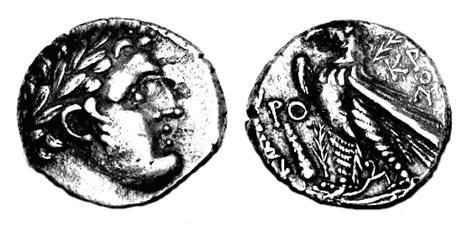
\includegraphics[width=\columnwidth]{images/Jerusalem-Tyrian-halfshekel.jpg}\caption{Jerusalem half-shekel of Tyrian type, 45\,A.D. On the obverse we see Melkhart, god of the Phoenicians, corresponding to the Greek Hercules. The reverse shows the eagle and the letters ``KP''. The meaning of ``KP'' is unknown, but this abbreviation is only present in the coins minted outside Tyre.}\end{figure}}
\vs p173 1:4 These temple money\hyp{}changers not only conducted a regular banking business for profit in the exchange of more than 20 sorts of money which the visiting pilgrims would periodically bring to Jerusalem, but they also engaged in all other kinds of transactions pertaining to the banking business. Both the temple treasury and the temple rulers profited tremendously from these commercial activities. It was not uncommon for the temple treasury to hold upwards of \$10,000,000 while the common people languished in poverty and continued to pay these unjust levies.
\vs p173 1:5 \pc In the midst of this noisy aggregation of money\hyp{}changers, merchandisers, and cattle sellers, Jesus, on this Monday morning, attempted to teach the gospel of the heavenly kingdom. He was not alone in resenting this profanation of the temple; the common people, especially the Jewish visitors from foreign provinces, also heartily resented this profiteering desecration of their national house of worship. At this time the Sanhedrin itself held its regular meetings in a chamber surrounded by all this babble and confusion of trade and barter.
\vs p173 1:6 As Jesus was about to begin his address, two things happened to arrest his attention. At the money table of a near\hyp{}by exchanger a violent and heated argument had arisen over the alleged overcharging of a Jew from Alexandria, while at the same moment the air was rent by the bellowing of a drove of some one hundred bullocks which was being driven from one section of the animal pens to another. As Jesus paused, silently but thoughtfully contemplating this scene of commerce and confusion, close by he beheld a simple\hyp{}minded Galilean, a man he had once talked with in Iron, being ridiculed and jostled about by supercilious and would\hyp{}be superior Judeans; and all of this combined to produce one of those strange and periodic uprisings of indignant emotion in the soul of Jesus.
\vs p173 1:7 To the amazement of his apostles, standing near at hand, who refrained from participation in what so soon followed, Jesus stepped down from the teaching platform and, going over to the lad who was driving the cattle through the court, took from him his whip of cords and swiftly drove the animals from the temple. But that was not all; he strode majestically before the wondering gaze of the thousands assembled in the temple court to the farthest cattle pen and proceeded to open the gates of every stall and to drive out the imprisoned animals. By this time the assembled pilgrims were electrified, and with uproarious shouting they moved toward the bazaars and began to overturn the tables of the money\hyp{}changers. In less than five minutes all commerce had been swept from the temple. By the time the near\hyp{}by Roman guards had appeared on the scene, all was quiet, and the crowds had become orderly; Jesus, returning to the speaker’s stand, spoke to the multitude: \textcolour{ubdarkred}{“You have this day witnessed that which is written in the Scriptures: ‘My house shall be called a house of prayer for all nations, but you have made it a den of robbers.’”}\tunemarkup{private}{\begin{figure}[H]\centering\includegraphics[width=\tunemarkup{pgkoboaurahd}{0.8}\columnwidth]{images/Money-Changers.jpg}\caption{Jesus Casts Out The Money\hyp{}Changers by William Hole}\end{figure}}
\vs p173 1:8 But before he could utter other words, the great assembly broke out in hosannas of praise, and presently a throng of youths stepped out from the crowd to sing grateful hymns of appreciation that the profane and profiteering merchandisers had been ejected from the sacred temple. By this time certain of the priests had arrived on the scene, and one of them said to Jesus, “Do you not hear what the children of the Levites say?” And the Master replied, \textcolour{ubdarkred}{“Have you never read, ‘Out of the mouths of babes and sucklings has praise been perfected’?”} And all the rest of that day while Jesus taught, guards set by the people stood watch at every archway, and they would not permit anyone to carry even an empty vessel across the temple courts.
\vs p173 1:9 \pc When the chief priests and the scribes heard about these happenings, they were dumbfounded. All the more they feared the Master, and all the more they determined to destroy him. But they were nonplussed. They did not know how to accomplish his death, for they greatly feared the multitudes, who were now so outspoken in their approval of his overthrow of the profane profiteers. And all this day, a day of quiet and peace in the temple courts, the people heard Jesus’ teaching and literally hung on his words.
\vs p173 1:10 This surprising act of Jesus was beyond the comprehension of his apostles. They were so taken aback by this sudden and unexpected move of their Master that they remained throughout the whole episode huddled together near the speaker’s stand; they never lifted a hand to further this cleansing of the temple. If this spectacular event had occurred the day before, at the time of Jesus’ triumphal arrival at the temple at the termination of his tumultuous procession through the gates of the city, all the while loudly acclaimed by the multitude, they would have been ready for it, but coming as it did, they were wholly unprepared to participate.
\vs p173 1:11 This cleansing of the temple discloses the Master’s attitude toward commercializing the practices of religion as well as his detestation of all forms of unfairness and profiteering at the expense of the poor and the unlearned. This episode also demonstrates that Jesus did not look with approval upon the refusal to employ force to protect the majority of any given human group against the unfair and enslaving practices of unjust minorities who may be able to entrench themselves behind political, financial, or ecclesiastical power. Shrewd, wicked, and designing men are not to be permitted to organize themselves for the exploitation and oppression of those who, because of their idealism, are not disposed to resort to force for self\hyp{}protection or for the furtherance of their laudable life projects.
\usection{Challenging the Master’s Authority}
\vs p173 2:1 On Sunday the triumphal entry into Jerusalem so overawed the Jewish leaders that they refrained from placing Jesus under arrest. Today, this spectacular cleansing of the temple likewise effectively postponed the Master’s apprehension. Day by day the rulers of the Jews were becoming more and more determined to destroy him, but they were distraught by two fears, which conspired to delay the hour of striking. The chief priests and the scribes were unwilling to arrest Jesus in public for fear the multitude might turn upon them in a fury of resentment; they also dreaded the possibility of the Roman guards being called upon to quell a popular uprising.
\vs p173 2:2 At the noon session of the Sanhedrin it was unanimously agreed that Jesus must be speedily destroyed, inasmuch as no friend of the Master attended this meeting. But they could not agree as to when and how he should be taken into custody. Finally they agreed upon appointing five groups to go out among the people and seek to entangle him in his teaching or otherwise to discredit him in the sight of those who listened to his instruction. Accordingly, about 14:00, when Jesus had just begun his discourse on “The Liberty of Sonship,” a group of these elders of Israel made their way up near Jesus and, interrupting him in the customary manner, asked this question: “By what authority do you do these things? Who gave you this authority?”
\vs p173 2:3 It was altogether proper that the temple rulers and the officers of the Jewish Sanhedrin should ask this question of anyone who presumed to teach and perform in the extraordinary manner which had been characteristic of Jesus, especially as concerned his recent conduct in clearing the temple of all commerce. These traders and money\hyp{}changers all operated by direct license from the highest rulers, and a percentage of their gains was supposed to go directly into the temple treasury. Do not forget that \bibemph{authority} was the watchword of all Jewry. The prophets were always stirring up trouble because they so boldly presumed to teach without authority, without having been duly instructed in the rabbinic academies and subsequently regularly ordained by the Sanhedrin. Lack of this authority in pretentious public teaching was looked upon as indicating either ignorant presumption or open rebellion. At this time only the Sanhedrin could ordain an elder or teacher, and such a ceremony had to take place in the presence of at least three persons who had previously been so ordained. Such an ordination conferred the title of “rabbi” upon the teacher and also qualified him to act as a judge, “binding and loosing such matters as might be brought to him for adjudication.”
\vs p173 2:4 The rulers of the temple came before Jesus at this afternoon hour challenging not only his teaching but his acts. Jesus well knew that these very men had long publicly taught that his authority for teaching was Satanic, and that all his mighty works had been wrought by the power of the prince of devils. Therefore did the Master begin his answer to their question by asking them a counter\hyp{}question. Said Jesus: \textcolour{ubdarkred}{“I would also like to ask you one question which, if you will answer me, I likewise will tell you by what authority I do these works. The baptism of John, whence was it? Did John get his authority from heaven or from men?”}
\vs p173 2:5 And when his questioners heard this, they withdrew to one side to take counsel among themselves as to what answer they might give. They had thought to embarrass Jesus before the multitude, but now they found themselves much confused before all who were assembled at that time in the temple court. And their discomfiture was all the more apparent when they returned to Jesus, saying: “Concerning the baptism of John, we cannot answer; we do not know.” And they so answered the Master because they had reasoned among themselves: If we shall say from heaven, then will he say, Why did you not believe him, and perchance will add that he received his authority from John; and if we shall say from men, then might the multitude turn upon us, for most of them hold that John was a prophet; and so they were compelled to come before Jesus and the people confessing that they, the religious teachers and leaders of Israel, could not (or would not) express an opinion about John’s mission. And when they had spoken, Jesus, looking down upon them, said, \textcolour{ubdarkred}{“Neither will I tell you by what authority I do these things.”}
\vs p173 2:6 \pc Jesus never intended to appeal to John for his authority; John had never been ordained by the Sanhedrin. Jesus’ authority was in himself and in his Father’s eternal supremacy.
\vs p173 2:7 In employing this method of dealing with his adversaries, Jesus did not mean to dodge the question. At first it may seem that he was guilty of a masterly evasion, but it was not so. Jesus was never disposed to take unfair advantage of even his enemies. In this apparent evasion he really supplied all his hearers with the answer to the Pharisees’ question as to the authority behind his mission. They had asserted that he performed by authority of the prince of devils. Jesus had repeatedly asserted that all his teaching and works were by the power and authority of his Father in heaven. This the Jewish leaders refused to accept and were seeking to corner him into admitting that he was an irregular teacher since he had never been sanctioned by the Sanhedrin. In answering them as he did, while not claiming authority from John, he so satisfied the people with the inference that the effort of his enemies to ensnare him was effectively turned upon themselves and was much to their discredit in the eyes of all present.
\vs p173 2:8 And it was this genius of the Master for dealing with his adversaries that made them so afraid of him. They attempted no more questions that day; they retired to take further counsel among themselves. But the people were not slow to discern the dishonesty and insincerity in these questions asked by the Jewish rulers. Even the common folk could not fail to distinguish between the moral majesty of the Master and the designing hypocrisy of his enemies. But the cleansing of the temple had brought the Sadducees over to the side of the Pharisees in perfecting the plan to destroy Jesus. And the Sadducees now represented a majority of the Sanhedrin.
\usection{Parable of the Two Sons}
\vs p173 3:1 As the cavilling Pharisees stood there in silence before Jesus, he looked down on them and said: \textcolour{ubdarkred}{“Since you are in doubt about John’s mission and arrayed in enmity against the teaching and the works of the Son of Man, give ear while I tell you a parable: A certain great and respected landholder had two sons, and desiring the help of his sons in the management of his large estates, he came to one of them, saying, ‘Son, go work today in my vineyard.’ And this unthinking son answered his father, saying, ‘I will not go’; but afterwards he repented and went. When he had found his older son, likewise he said to him, ‘Son, go work in my vineyard.’ And this hypocritical and unfaithful son answered, ‘Yes, my father, I will go.’ But when his father had departed, he went not. Let me ask you, which of these sons really did his father’s will?”}
\vs p173 3:2 And the people spoke with one accord, saying, “The first son.” And then said Jesus: \textcolour{ubdarkred}{“Even so; and now do I declare that the publicans and harlots, even though they appear to refuse the call to repentance, shall see the error of their way and go on into the kingdom of God before you, who make great pretensions of serving the Father in heaven while you refuse to do the works of the Father. It was not you, the Pharisees and scribes, who believed John, but rather the publicans and sinners; neither do you believe my teaching, but the common people hear my words gladly.”}
\vs p173 3:3 Jesus did not despise the Pharisees and Sadducees personally. It was their systems of teaching and practice which he sought to discredit. He was hostile to no man, but here was occurring the inevitable clash between a new and living religion of the spirit and the older religion of ceremony, tradition, and authority.
\vs p173 3:4 All this time the twelve apostles stood near the Master, but they did not in any manner participate in these transactions. Each one of the twelve was reacting in his own peculiar way to the events of these closing days of Jesus’ ministry in the flesh, and each one likewise remained obedient to the Master’s injunction to refrain from all public teaching and preaching during this Passover week.
\usection{Parable of the Absent Landlord}
\vs p173 4:1 When the chief Pharisees and the scribes who had sought to entangle Jesus with their questions had finished listening to the story of the two sons, they withdrew to take further counsel, and the Master, turning his attention to the listening multitude, told another parable:
\vs p173 4:2 \pc \textcolour{ubdarkred}{“There was a good man who was a householder, and he planted a vineyard. He set a hedge about it, dug a pit for the wine press, and built a watchtower for the guards. Then he let this vineyard out to tenants while he went on a long journey into another country. And when the season of the fruits drew near, he sent servants to the tenants to receive his rental. But they took counsel among themselves and refused to give these servants the fruits due their master; instead, they fell upon his servants, beating one, stoning another, and sending the others away empty\hyp{}handed. And when the householder heard about all this, he sent other and more trusted servants to deal with these wicked tenants, and these they wounded and also treated shamefully. And then the householder sent his favourite servant, his steward, and him they killed. And still, in patience and with forbearance, he dispatched many other servants, but none would they receive. Some they beat, others they killed, and when the householder had been so dealt with, he decided to send his son to deal with these ungrateful tenants, saying to himself, ‘They may mistreat my servants, but they will surely show respect for my beloved son.’ But when these unrepentant and wicked tenants saw the son, they reasoned among themselves: ‘This is the heir; come, let us kill him and then the inheritance will be ours.’ So they laid hold on him, and after casting him out of the vineyard, they killed him. When the lord of that vineyard shall hear how they have rejected and killed his son, what will he do to those ungrateful and wicked tenants?”}
\vs p173 4:3 \pc And when the people heard this parable and the question Jesus asked, they answered, “He will destroy those miserable men and let out his vineyard to other and honest farmers who will render to him the fruits in their season.” And when some of them who heard perceived that this parable referred to the Jewish nation and its treatment of the prophets and to the impending rejection of Jesus and the gospel of the kingdom, they said in sorrow, “God forbid that we should go on doing these things.”
\vs p173 4:4 Jesus saw a group of the Sadducees and Pharisees making their way through the crowd, and he paused for a moment until they drew near him, when he said: \textcolour{ubdarkred}{“You know how your fathers rejected the prophets, and you well know that you are set in your hearts to reject the Son of Man.”} And then, looking with searching gaze upon those priests and elders who were standing near him, Jesus said: \textcolour{ubdarkred}{“Did you never read in the Scripture about the stone which the builders rejected, and which, when the people had discovered it, was made into the cornerstone? And so once more do I warn you that, if you continue to reject this gospel, presently will the kingdom of God be taken away from you and be given to a people willing to receive the good news and to bring forth the fruits of the spirit. And there is a mystery about this stone, seeing that whoso falls upon it, while he is thereby broken in pieces, shall be saved; but on whomsoever this stone falls, he will be ground to dust and his ashes scattered to the four winds.”}
\vs p173 4:5 When the Pharisees heard these words, they understood that Jesus referred to themselves and the other Jewish leaders. They greatly desired to lay hold on him then and there, but they feared the multitude. However, they were so angered by the Master’s words that they withdrew and held further counsel among themselves as to how they might bring about his death. And that night both the Sadducees and the Pharisees joined hands in the plan to entrap him the next day.
\usection{Parable of the Marriage Feast}
\vs p173 5:1 After the scribes and rulers had withdrawn, Jesus addressed himself again to the assembled crowd and spoke the parable of the wedding feast. He said:
\vs p173 5:2 \pc \textcolour{ubdarkred}{“The kingdom of heaven may be likened to a certain king who made a marriage feast for his son and dispatched messengers to call those who had previously been invited to the feast to come, saying, ‘Everything is ready for the marriage supper at the king’s palace.’ Now, many of those who had once promised to attend, at this time refused to come. When the king heard of these rejections of his invitation, he sent other servants and messengers, saying: ‘Tell all those who were bidden, to come, for, behold, my dinner is ready. My oxen and my fatlings are killed, and all is in readiness for the celebration of the forthcoming marriage of my son.’ But again did the thoughtless make light of this call of their king, and they went their ways, one to the farm, another to the pottery, and others to their merchandise. Still others were not content thus to slight the king’s call, but in open rebellion they laid hands on the king’s messengers and shamefully mistreated them, even killing some of them. And when the king perceived that his chosen guests, even those who had accepted his preliminary invitation and had promised to attend the wedding feast, had finally rejected his call and in rebellion had assaulted and slain his chosen messengers, he was exceedingly wroth. And then this insulted king ordered out his armies and the armies of his allies and instructed them to destroy these rebellious murderers and to burn down their city.}
\vs p173 5:3 \textcolour{ubdarkred}{“And when he had punished those who spurned his invitation, he appointed yet another day for the wedding feast and said to his messengers: ‘They who were first bidden to the wedding were not worthy; so go now into the parting of the ways and into the highways and even beyond the borders of the city, and as many as you shall find, bid even these strangers to come in and attend this wedding feast.’ And then these servants went out into the highways and the out\hyp{}of\hyp{}the\hyp{}way places, and they gathered together as many as they found, good and bad, rich and poor, so that at last the wedding chamber was filled with willing guests. When all was ready, the king came in to view his guests, and much to his surprise he saw there a man without a wedding garment. The king, since he had freely provided wedding garments for all his guests, addressing this man, said: ‘Friend, how is it that you come into my guest chamber on this occasion without a wedding garment?’ And this unprepared man was speechless. Then said the king to his servants: ‘Cast out this thoughtless guest from my house to share the lot of all the others who have spurned my hospitality and rejected my call. I will have none here except those who delight to accept my invitation, and who do me the honour to wear those guest garments so freely provided for all.’”}
\vs p173 5:4 \pc After speaking this parable, Jesus was about to dismiss the multitude when a sympathetic believer, making his way through the crowds toward him, asked: “But, Master, how shall we know about these things? how shall we be ready for the king’s invitation? what sign will you give us whereby we shall know that you are the Son of God?” And when the Master heard this, he said, \textcolour{ubdarkred}{“Only one sign shall be given you.”} And then, pointing to his own body, he continued, \textcolour{ubdarkred}{“Destroy this temple, and in three days I will raise it up.”} But they did not understand him, and as they dispersed, they talked among themselves, saying, “Almost 50 years has this temple been in building, and yet he says he will destroy it and raise it up in 3 days.” Even his own apostles did not comprehend the significance of this utterance, but subsequently, after his resurrection, they recalled what he had said.
\vs p173 5:5 About 16:00 Jesus beckoned to his apostles and indicated that he desired to leave the temple and to go to Bethany for their evening meal and a night of rest. On the way up Olivet Jesus instructed Andrew, Philip, and Thomas that, on the morrow, they should establish a camp nearer the city which they could occupy during the remainder of the Passover week. In compliance with this instruction the following morning they pitched their tents in the hillside ravine overlooking the public camping park of Gethsemane, on a plot of ground belonging to Simon of Bethany.
\vs p173 5:6 Again it was a silent group of Jews who made their way up the western slope of Olivet on this Monday night. These twelve men, as never before, were beginning to sense that something tragic was about to happen. While the dramatic cleansing of the temple during the early morning had aroused their hopes of seeing the Master assert himself and manifest his mighty powers, the events of the entire afternoon only operated as an anticlimax in that they all pointed to the certain rejection of Jesus’ teaching by the Jewish authorities. The apostles were gripped by suspense and were held in the firm grasp of a terrible uncertainty. They realized that only a few short days could intervene between the events of the day just passed and the crash of an impending doom. They all felt that something tremendous was about to happen, but they knew not what to expect. They went to their various places for rest, but they slept very little. Even the Alpheus twins were at last aroused to the realization that the events of the Master’s life were moving swiftly toward their final culmination.
\quizlink
